% This is samplepaper.tex, a sample chapter demonstrating the
% LLNCS macro package for Springer Computer Science proceedings;
% Version 2.21 of 2022/01/12
%
\documentclass[runningheads]{llncs}
%
\usepackage[T1]{fontenc}
% T1 fonts will be used to generate the final print and online PDFs,
% so please use T1 fonts in your manuscript whenever possible.
% Other font encondings may result in incorrect characters.
%
\usepackage{graphicx}
\usepackage{amsmath}
\usepackage{amssymb}
\usepackage{listings}
\usepackage{xcolor}
\usepackage{listings}
\usepackage{pgfplots}
\usepackage{array}
\usepackage{booktabs}
\usepackage{tikz}
% Used for displaying a sample figure. If possible, figure files should
% be included in EPS format.
%
% If you use the hyperref package, please uncomment the following two lines
% to display URLs in blue roman font according to Springer's eBook style:
%\usepackage{color}
%\renewcommand\UrlFont{\color{blue}\rmfamily}
%\urlstyle{rm}
%
\usetikzlibrary{shapes.geometric, arrows}
\tikzstyle{startstop} = [rectangle, rounded corners, minimum width=3cm, minimum height=0.6cm,text centered, draw=black, fill=red!30]
\tikzstyle{process} = [rectangle, minimum width=4cm, minimum height=0.8cm, text centered, draw=black, fill=orange!30]
\tikzstyle{decision} = [diamond, minimum width=3cm, minimum height=0.4cm, text centered, draw=black, fill=blue!30]
\tikzstyle{arrow} = [thick,->,>=stealth]

\lstdefinelanguage{solidity}{
  backgroundcolor=\color{pink!20},
  keywords={contract, function, public, int},
  keywordstyle=\bfseries\color{blue},
  commentstyle=\itshape\color{green!40!black},
  basicstyle=\ttfamily,
  morecomment=[l]{//},
  morecomment=[s]{/*}{*/},
  morestring=[b]",
  sensitive=true
}
\begin{document}
%
\title{Gas-Efficient Parameter Verification for Blockchain Smart Contracts Using Off-Chain Validators}
%
\titlerunning{Off-Chain Parameter Verification Approach: Gas-Efficient}
% If the paper title is too long for the running head, you can set
% an abbreviated paper title here
%
%\author{Thi Thu Ha Doan\orcidID{0000-0001-7524-4497}\and Peter Thiemann\orcidID{0000-0002-9000-1239}}
%
%\authorrunning{Ha Doan, P. Thiemann}
% First names are abbreviated in the running head.
% If there are more than two authors, 'et al.' is used.
%
%\institute{University of Freiburg, Germany \\
%  \email{\{doanha,thiemann\}@informatik.uni-freiburg.de}}
%
\maketitle              % typeset the header of the contribution
%
\begin{abstract}
In certain blockchain scenarios, verifying the properties of parameters may require significant gas costs or be infeasible due to gas limits. This study proposes a distributed verification protocol to address these challenges. The core concept involves offloading the verification process to validators, who attempt to find counterexamples or proofs off-chain. If a counterexample is discovered, it can be submitted for re-verification on-chain. If validated, the parameter is discarded; otherwise, the correctness of the parameter is guaranteed through a proof-of-work incentive mechanism, encouraging validators to participate in the distributed verification process. To implement these ideas, we propose a practical model that tackles potential security concerns. We developed a prototype of the protocol and conducted a cost analysis, demonstrating its gas efficiency and practical utility.
\keywords{blockchain, off-chain verification, gas optimization, proof-of-work, distributed verification}
\end{abstract}
%
%
%
\section{Introduction}
\label{sec:introduction}
\lstset{language=solidity}
A smart contract \cite{szabo1997smartcontracts,eth-whitepaper,tezos-whitepaper} is a critical component of blockchain technology, with applications ranging from simple tasks like auctions to more complex systems such as decentralized markets. However, broader adoption of smart contracts faces challenges, with gas costs being among the most significant. Every computation performed by a smart contract on the blockchain incurs a cost, as each unit of computation and storage consumed by an algorithm must be paid for due to the burden it places on the system \cite{eth-whitepaper,eth-yellowpaper,gas-cost}.

When users (or other contracts) invoke a function in a smart contract, they must provide input data, known as parameters. In many cases, these parameters require verification. For instance, to minimize gas costs, an application might perform some computation off-chain and submit the result as a parameter to a smart contract. Such computations typically assert certain properties of the submitted parameters.

Another scenario involves interactions with external data sources. Since smart contracts cannot directly access off-chain data, blockchain oracles \cite{blockchain-oracles,oracle-patterns,astraea,chainlink-whitepaper} supply this information. When external data becomes available, an oracle invokes a smart contract with the relevant information.

However, while the contract should leverage off-chain computations or external data and assume that the submitted parameters are valid, there is a risk that off-chain computations could be incorrect, submitting invalid parameters, or that oracles could provide faulty data. Therefore, a mechanism is needed to verify these assumptions before the contract begins execution.

Unfortunately, most current applications cannot efficiently verify complex parameters on-chain due to the high gas costs associated with such computations. This limitation restricts many applications that require parameter verification during smart contract execution. The primary goal of this paper is to propose an approach that validates complex parameter assumptions while minimizing gas costs, without sacrificing computational efficiency.

Consider a contract that takes a prime number as a parameter:
\begin{lstlisting}[numbers=none]
contract Example {
  function (int p) public { 
    // assume p is prime 
  ... }}
\end{lstlisting}
This assumption can be expressed as an explicit assertion in predicate logic:
\begin{gather*}
\label{eq1}
  (\forall n) (2 \leq n \leq \sqrt{p}) \Rightarrow (p \mathbin{\%} n) \ne 0
\end{gather*}
Checking the validity of this assumption requires a loop in the contract. The test would take \(O(\sqrt{p})\) time (assuming constant time for computing the remainder) and produce extra cost linear in \(\sqrt{p}\).

Similarly, consider a contract that requires a sorted array \(a\)  of the size \(n\)  of integers as input. 
%\begin{lstlisting}[numbers=none]
%contract Sorted {
%  function find (int[100] a, int v) public {
%    // assume a is sorted
%  ...}}
%\end{lstlisting}
The explicit assertion would be:
\begin{gather*}\label{}
  (\forall k) (0\leq k <n) \Rightarrow a[k] \leq a[k+1]
\end{gather*}
This check can be performed in \(O(1)\) time, but the associated constant factor makes it costly.

However, we could do better by recruiting the validators of the contract for a distributed effort to find a counterexample off-chain. To this end, we consider the negation of these assertions. 

For the prime number example, the negation is:
\begin{gather*}\label{}
  (\exists n) (2 \leq n \leq \sqrt{p}) \wedge (p \mathbin{\%} n) = 0
\end{gather*}
This assertion can be checked pointwise by having each validator independently choose a random \(n\) fulfilling \(2 \leq n \leq \sqrt{p}\) and checking whether \((p \mathbin{\%} n) = 0\). If the remainder is \(0\), the validator has found a counterexample and submits its veto to the on-chain contract, which then verifies the counterexample. If valid, the contract halts further execution with that parameter. If no counterexample is found, \(p\) is accepted, assuming other validators have checked other points.

For the sorted array example, the negation is:
\begin{gather*}\label{}
  (\exists k) (0\leq k <n) \wedge a[k] > a[k+1]
\end{gather*}
Again, we can have every validator generate a random number \(k\). If the condition is true for such \(k\), the validator has found a counterexample for the sortedness of the array. Otherwise, the validator relies on others to check different indices.

Instead of looping and checking all points on-chain, only one or some points are checked. The checking process can be performed off-chain with no gas cost, and only the result of the verification process needs to be validated on-chain. By shifting much of the verification off-chain, our propsed approach significantly reduces gas costs, as only counterexample verification occurs on-chain.

This approach substantially reduces on-chain gas costs by moving most of the verification work off-chain. However, it introduces challenges related to incentivizing validators, ensuring the cost-effectiveness of on-chain verifications, and providing correctness guarantees when no counterexamples are found.

To address these challenges, we propose a proof-of-work-based incentive mechanism that encourages validator participation and ensures that parameters meet the desired properties with a high level of confidence. The detailed methodology of this approach are discussed in Section \ref{sec:offchain-distributed-verification-approach}.

To realize our novel approach, we propose a practical model that implements the approach and addresses security concerns. We then develop a prototype of the practical model for a decentralized marketplace application using Solidity on the Ethereum blockchain.

The contributions of this paper include:
\begin{itemize}
    \item A novel approach for verifying computationally expensive parameters (in terms of gas cost) for smart contracts on the blockchain.
    \item A proof-of-work-based incentive mechanism that motivates validators to participate in the distributed verification process and ensures the correctness of the submitted parameter with a high expected probability.
    \item A practical model that realizes the proposed novel approach, along with a prototype implementation of the model for a Solidity smart contract application on the Ethereum blockchain.
\end{itemize}


The paper is structured as follows: The next section defines the parameter verification problems and presents use cases. Section \ref{sec:offchain-distributed-verification-approach} proposes the novel approach, while Section \ref{sec:practical-model} introduces its practical model. Section \ref{sec:gas-cost-analysis} analyzes the gas costs, comparing our proposed approach with the on-chain method. Section \ref{sec:prototype-implementation} details the prototype implementation. Section \ref{sec:related-work} discusses related work, and Section \ref{sec:conclusion} concludes the paper.
\section{Parameter Assertion Verification On-chain}
\label{sec:parameter-assertion-verification-onchain}
Our work targets parameters that are computationally expensive to verify on-chain, particularly when verification involves loops within the contract. We focus on assertions that can be expressed using universal or existential quantifiers.
\subsection{Parameter Assertion Formalization}
\paragraph{Universal Quantifier Formalization}
An parameter assertion can be formalized using the universal quantifier over the domain \(A\) as:
\begin{equation} \label{eq:1}
    \forall a \in A, \, P(a)
\end{equation}
For multiple domains:
\begin{equation} \label{eq:2}
    \forall a \in A, \, \forall b \in B, \, \dots, \, P(a, b, \dots)
\end{equation}

\paragraph{Existential Quantifier Formalization}
For assertions involving the existence of an element, we use existential quantifiers:
\begin{equation} \label{eq:3}
    \exists a \in A, \, P(a)
\end{equation}
Extended to multiple domains:
\begin{equation} \label{eq:4}
    \exists a \in A, \, \exists b \in B, \, \dots, \, P(a, b, \dots)
\end{equation}
\subsection{On-chain Verification}
Verifying these assertions on-chain involves iterating over the domain \(A\)\footnote{For multiple domains, the verification process requires iterating over all domains} within the contract. For formula \ref{eq:1}, the verification is expressed as: \(   \bigwedge_{a \in A} P(a)\).

´For the existential quantifier formalization as in formula \ref{eq:3}, verification requires iterating over \(A\) until an element \(a\) is found that satisfies \(P\): \(\bigvee_{a \in A} P(a)\).

When \(A\) is large or \(P\) is complex to evaluate, this process can incur significant gas costs or even become infeasible due to gas limits. Given the current high gas prices, this could result in substantial expenses.
\subsection{Use Cases}
Smart contract languages like Solidity \cite{solidity}, Vyper \cite{vyper}, Michelson \cite{michelson,michelson1}, and Plutus \cite{plutus} support common data types such as numbers, booleans, strings, bytes, arrays, sets. Many properties of these types use quantifiers, requiring loops for verification but can often be disproven by a counterexample or proven formally. Key properties for each type are outlined below:
\paragraph{\textbf{Numbers}}
Number types have some properties that are vital in cryptographic applications, such as primality and coprimeness. %For instance, the condition for two numbers \(a\) and \(b\) to be coprime is:
%\begin{equation*}
%(\forall n) \ (2 \leq n \leq \min(a, b)) \Rightarrow \neg((a \mod n = 0) \wedge (b \mod n = 0))
%\end{equation*}
\paragraph{\textbf{Booleans}}
SAT problems determine if there is an assignment of variables that makes a formula \( F \) in propositional logic true. Verifying whether a given assignment satisfies \( F \), typically in Conjunctive Normal Form (CNF), involves iterating over variables and clauses. While finding a satisfying assignment is NP-complete, verifying one takes \( O(n \times m) \), where \( n \) is the number of clauses and \( m \) is the number of variables.
\paragraph{\textbf{Strings}}
String properties that require iteration include uniqueness, character set membership, lexicographical order, pattern matching, and forbidden substrings. %For example, verifying that a string \(s\) lacks a forbidden substring \(f\) of length \(k\) is expressed as:
%\begin{gather*}
%(\forall i) \ (0 \leq i \leq n - k) \Rightarrow s[i, i+1, \dots, i+k-1] \neq f
%\end{gather*}
\paragraph{\textbf{Bytes}}
Verifying byte arrays often involves loops for properties such as uniformity, sorted order, specific byte patterns, uniqueness, valid range, and alternating patterns. For instance, to check if all bytes in an array \(b\) are within a range \([l, u]\), the condition is:
\begin{gather*}
(\forall i) \ (0 \leq i \leq n) \Rightarrow l \leq b[i] \leq u
\end{gather*}
\paragraph{\textbf{Arrays (or Lists)}}
Common properties of arrays include sortedness, uniqueness, boundedness, monotonicity, symmetry, cyclic structure, and constant values. %A tree-based structure like a max-heap, where each parent node is greater than or equal to its children, can be checked as:
Tree-based structures like heaps can also be built from arrays, with properties such as the heap property. For example, in a max-heap, each parent node is greater than or equal to its children. This property can be expressed as:
\begin{gather*}
(\forall i) \ a[i] \geq a[2i+1] \land a[i] \geq a[2i+2]
\end{gather*}
\paragraph{\textbf{Sets}}
Set properties like subset verification, disjoint sets, element uniqueness, set equality, and set intersection often require loops. For example, verifying that two sets \(A\) and \(B\) share at least one element can be expressed as:
\begin{gather*}
(\exists a \in A) (\exists b \in B)\ a = b
\end{gather*}
%Such properties can be computationally expensive for large sets.
\section{Gas-Efficient Off-chain Distributed Parameter Verification Approach}
\label{sec:offchain-distributed-verification-approach}
\subsection{The Outline of the Approach}
We propose a novel approach for verifying parameter assertions in blockchain-based smart contracts by offloading the verification process off-chain and submitting only the results for on-chain re-verification. 
Our approach leverages the principle that assertions with universal quantifiers can be disproven by counterexamples, while those with existential quantifiers can be proven with valid proofs. These counterexamples or proofs act as checkpoints, representing specific elements within the domain.

The outline of our approach is as follows:
\paragraph{\textbf{Determine the checkpoint formula.}}
The first step is to establish the checkpoint formula used to identify counterexamples or proofs. For assertions with universal quantifiers, the checkpoint formula is the negation of the original assertion and is expressed using an existential quantifier as follows: 
\begin{gather}
\label{eq:9}
(\exists a \in A) \ \neg P(a)
\end{gather}
For assertions over multiple domains, the checkpoint formula becomes:
\begin{gather}
\label{eq:10}
(\exists a \in A) (\exists b \in B) \dots  \neg P(a, b, \dots)
\end{gather}
In the case of existential quantifier assertions, the checkpoint formula remains the same as the original assertion.
\paragraph{\textbf{Off-chain distributed effors.}} These checkpoint formulas are distributed to validators, who then work off-chain to find counterexamples or proofs by identifying some \( a \in A \) that satisfies the checkpoint formula. For universal quantifiers, this involves finding \( a \) where \( \neg P(a) \) holds, while for existential quantifiers, it requires finding \( a \) where \( P(a) \) is true.
\paragraph{\textbf{On-chain re-verification.}} After finding a counterexample or proof involving an element \( a \), the validator submits it to the blockchain for on-chain re-verification by evaluating \( \neg P(a) \) or \( P(a) \). For universal quantifiers, a verified counterexample invalidates the assertion; otherwise, it is assumed valid if other points are verified by other validators. For existential quantifiers, the assertion remains invalid until a proof is submitted and verified on-chain.
\paragraph{\textbf{Incentivization Mechanism.}} Validators are incentivized to find counterexamples or provide proofs, which require computational resources. Since counterexamples are rare (as callers avoid submitting invalid parameters), confidence in correctness grows with more validator attempts at different checkpoints. Thus, incentivization is crucial for ensuring correctness in the absence of counterexamples.Validators are rewarded for both finding counterexamples and contributing computational proofs, with  counterexample discovery prioritized through higher rewards. 

Overall, the approach reduces the blockchain's computational load while preserving contract integrity. By verifying only specific checkpoints instead of full on-chain verification, it lowers the blockchain's burden and reduces gas costs.
\subsection{Proof-of-Work-Based Incentivization Mechanism}
The computational effort is represented by a computation proof, submitted on-chain by the validator to claim a reward. This incentivizes participation in distributed verification, ensuring thorough validation even without finding counterexamples.

Challenges include: (1) rechecking counterexamples and computation efforts on-chain at low gas costs, (2) ensuring sufficient checkpoints are performed before rewarding computation, guaranteeing a probability of correctness, and (3) verifying that validators perform the checkpoint formula off-chain when no counterexample is found.

To address these, we propose a proof-of-work-based mechanism. Using the proof-of-work concept \cite{dwork1992pow,nakamoto2008bitcoin}, a target hash \( t \) sets the difficulty level for earning rewards. Each verification introduces a target hash, and the validator performs the checkpoint, computing a hash. The validator’s goal is to find a counterexample or produce a hash  that is less than or equal to \( t \).
\subsubsection{Introduce a seed} 
Let the element \( a \in A \) be where the assertion fails, either as a counterexample or as the computation proof found. To recheck this on-chain at a reasonable gas cost, it should be submitted as the element \( a \in A \) or as an indication of it. The on-chain re-verification then simply evaluates \( \neg P(a) \). The next challenge is generating a random hash for each checkpoint computation to provide computational proof. We address these by introducing a seed \( s \) in each verification process.


Let \( n \) denote the size of the domain \( A \), where \( n = |A| \) and \(|A|\) is the number of elements in \( A \). Each number \( i \) in the range \([1, n]\) corresponds to an element in \( A \), such that \( a = A[i] \), where \( A[i] \) denotes the \( i \)-th element of \( A \).

We introduce a seed \( s \), a random number \( s \in \mathbb{N} \). The seed \( s \) is reduced modulo \( n \) to obtain \( i \), which is then associated with an element \( a \) in \( A \):
\begin{equation}
\label{eq:11}
i = (s \mod n) + 1
\end{equation}
\subsubsection{Estimate the Number of Seeds:} To ensure a sufficient number of checkpoints are checked before finding a computational proof, we estimate the number of seeds required to find a counterexample with the desired probability of correctness \cite{ross2014probability,feller1968probability}.

Assuming the unsatisfied element is only the first element \( a_0 \) in \( A \) and the number of seeds is \( m \), each seed independently has a probability of \( \frac{1}{n} \) to detect the issue and \( \frac{n-1}{n} \) not to. If each seed associated with an element \( a \) in \( A \) is chosen uniformly and independently, the probability that no seed checks \( a_0 \) approaches 0 as \( m \) increases:
\begin{gather*}
\lim_{m \to \infty} \frac{(n-1)^m}{n^m} = \lim_{m \to \infty} \left( \frac{n-1}{n} \right)^m = 0
\end{gather*}

To determine the number of seeds needed based on the expected probability of detecting a problem, we define \( p \) as the expected probability of finding at least one counterexample. 
\begin{itemize}
    \item The probability of a single seed failing to find a counterexample is \( \frac{n-1}{n} \).
    \item The probability of all \( m \) seeds failing is \( \left( \frac{n-1}{n} \right)^m \).
    \item Thus, the probability of at least one seed finding a counterexample is:
\begin{gather*}
  p = 1 - \left( \frac{n-1}{n} \right)^m
\end{gather*}
\end{itemize}
Solving for \( m \):
\begin{equation}
\label{eq:12}
m = \frac{\ln(1 - p)}{\ln\left( \frac{n-1}{n} \right)}
\end{equation}

Therefore, the number of seeds required to achieve the expected probability \( p \) is at least \( m \). Note that \( p \) represents the probability when only one validator participates. As more validators are involved, the probability of discovering a counterexample increases.
\subsubsection{Set up the Target Hash:}
The number of seeds \( m \) can be used to set up the target hash \cite{nakamoto2008bitcoin,bonneau2015sok}. The target hash \( t \) is calculated based on a desired difficulty level. In proof-of-work systems, difficulty is typically adjusted to ensure that the average effort to find a valid hash matches the desired rate. The target hash \( t \) is often determined by taking the maximum possible hash value and dividing it by the difficulty level.

Given the expected number of seeds, the difficulty level \( D \) can be adjusted accordingly. Typically, \( D \) is set to ensure that a valid hash is found approximately once every \( m \) trials. If we want the probability of finding a valid hash to be \( \frac{1}{m} \), then \( D \) is set to \( m \):
\begin{equation}
\label{eq:13}
t = \frac{H_{\text{max}}}{m}
\end{equation}
Where \( H_{\text{max}} \) is the maximum possible hash value, and \( m \) is the difficulty level, adjusted based on the expected number of trials.
\subsubsection{Conduct a Computation Hash:} To ensure a computational proof includes the negation check, the checkpoint formula is integrated into the proof process, requiring validators to execute it as part of producing the proof.

For each element \( a \), let \(\pi_{P_{a}}\) represent the components for evaluating the checkpoint \(\neg P(a)\). The computation hash combines the seed \( s \) and \(\pi_{P_{a}}\) to ensure validation.

\begin{equation}
\label{eq:14}
t_s = \text{hash}(s, \pi_{P_{a}})
\end{equation}
where \(\text{hash}\) is a cryptographic hash function.

Assertions in smart contract languages are represented as predicate logic expressed through Boolean formulas. These formulas are composed of relational operators like \( =, \neq, >, <, \geq, \leq \) and logical operators such as \( \neg, \land, \lor \), along with corresponding expressions.

Thus, \(\pi_{P_{a}}\) denotes the set of expressions used to evaluate \(P_a\):
\begin{equation*}
\pi_{P_{a}} = \{ e_1, e_2, \ldots \}
\end{equation*}
where \(e_i\) are the expressions contributing to the computation of \(P_a\).
\subsection{Off-chain Distributed Verification}
For assertions using an existential quantifier, validation is straightforward: validators find a proof off-chain and submit it on-chain for re-verification. If valid, the parameter is confirmed, and the validator is rewarded.

For universal quantifier assertions, the process is more complex. The size \( n \) of the domain \( A \) is calculated, and the target hash is computed based on the expected probability of correctness. Validators generate approximately \( m \) seeds to find either a counterexample or a computational proof, confirming or invalidating the parameter.

As shown in Fig. \ref{fig:find_seed}, validators generate a seed \( s \) and perform the checkpoint until they find a counterexample or computation proof. They then submit the result on-chain to claim their reward.

Both counterexamples and proofs are encoded by the seed, enabling on-chain verification. If successful, the validator receives the reward.
\begin{figure}[t]
    \centering
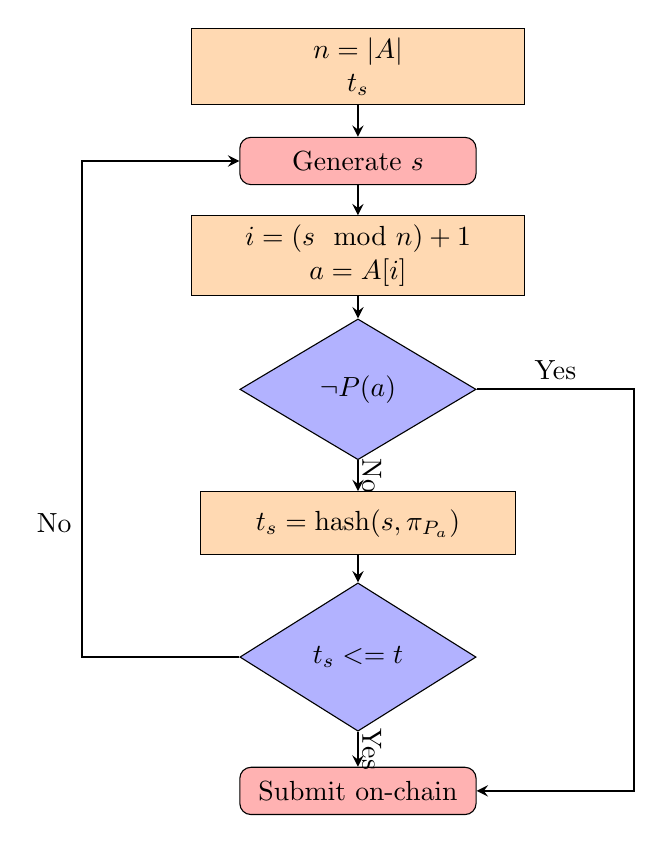
\begin{tikzpicture}[node distance=1.2cm]
    % Nodes
    \node (calc_n) [process] {\parbox{4cm}{\centering $n = |A|$ \\ $t_s$}}; 
    \node (start) [startstop, below of=calc_n] {Generate $s$};
    \node (calc_i) [process, below of=start] {\parbox{4cm}{\centering $i = (s \mod n) + 1$ \\ $a = A[i]$}};
    \node (counterexample) [decision, below of=calc_i, yshift=-0.5cm] {$\neg P(a)$};
    \node (calc_hash) [process, below of=counterexample, yshift=-0.5cm] {$t_s = \text{hash}(s,\pi_{P_{a}})$};
    \node (compare) [decision, below of=calc_hash, yshift=-0.5cm] {$t_s <= t$};
    \node (submit) [startstop, below of=compare, yshift=-0.5cm] {Submit on-chain};
    % Arrows
    \draw [arrow] (calc_n) -- (start);
    \draw [arrow] (start) -- (calc_i);
    \draw [arrow] (calc_i) -- (counterexample);
    \draw [arrow] (counterexample) -- node[midway, above, sloped, anchor=center, yshift=0.5em] {No} (calc_hash);
    \draw [arrow] (calc_hash) -- (compare);
    \draw [arrow] (compare) -- (submit) node[midway, above, sloped, anchor=center, yshift=0.5em] {Yes};
	\draw [arrow] (counterexample.east) -| node[pos=0.25, above] {Yes} ([xshift=2cm]submit.east) |- (submit);
	\draw [arrow] (compare.west) -| node[pos=0.75, left] {No} ([xshift=-2cm]counterexample.west) |- (start);
\end{tikzpicture}
\caption{Finding a reward seed.}
\label{fig:find_seed}
\end{figure}
\subsection{On-chain Re-verification}
Given a submitted seed \( s \), the on-chain contract verifies if it produces a counterexample or a valid computational proof for a reward. The process involves: (1) Compute \( n \), the size of the domain \( A \), (2) Identify the target value \( t \), (3) Determine \( i \in [1, n] \) from \( s \) using modulo, and associate it with the element \( a \in A \), (4) Check \( \neg P(a) \) for a counterexample, (5) If none, compute the hash \( t_s \) from \( s \), and (6) Compare \( t_s \) to the target hash \( t \) to check reward eligibility.

The contract either identifies a counterexample or computes a hash based on \( s \) and \( \neg P(a) \), then compares it to \( t \) to decide if a reward is given.
\section{Practical Model}
\label{sec:practical-model}
\subsection{Security Risks}
Off-chain distributed verification presents several security risks:
\begin{enumerate}
\item Denial-of-service (DoS) attacks: Attackers can flood the system with invalid parameters, causing congestion and disrupting operations.
\item Front-running attacks: Attackers can monitor the mempool to intercept seeds representing counterexamples or proofs, stealing rewards.
\item Caller exploitation: Callers may privately run negation checks to (1) claim rewards before others or (2) fake computation proofs before a counterexample is found.
\item Reward manipulation: Validators might resubmit counterexamples or proofs multiple times to manipulate and multiply rewards.
\end{enumerate}
\subsection{Architectural Overview}
This section presents a practical model that combines theoretical principles and addresses security concerns. The architecture is shown in Figure \ref{fig.architect}.
The model has two key entities: the on-chain assertion contract and the off-chain validator program. 
\paragraph{On-chain assertion contract.} The contract includes two essential functions: (1) \( submitParameter \), used by callers to submit parameters for validation, and (2) \( claimReward \), which accepts a seed and determines if it results in a counterexample, a reward, or no reward.
\paragraph{Off-chain Validator Program.}
The off-chain program must use the same \( claimReward \) function for finding counterexamples or proofs and assist validators in finding seeds for rewards. Events like parameter submissions, counterexamples, or proofs can be broadcast via event emission for real-time monitoring.

The owner deploys the on-chain contract and makes the off-chain program available by either (1) storing the code in a repository or (2) broadcasting it via messaging systems like Waku in Ethereum for local storage by validators.
\paragraph{Storage.}
When a parameter is submitted for verification, the following should be stored: (1) The parameter itself, or if too large, only its hash, which is sufficient for validation, and (2) the timestamp of when the parameter was submitted.
\begin{figure}
\centering
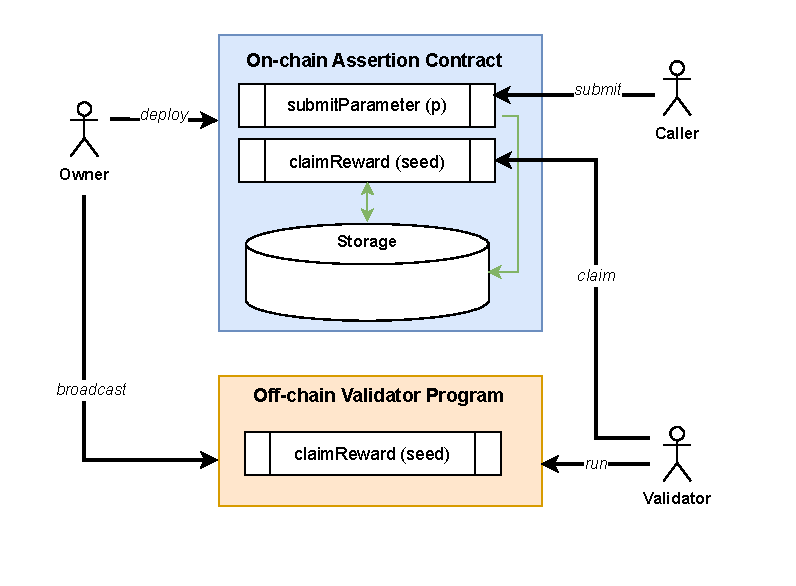
\includegraphics[scale=.6]{assertion1}
\caption{The architecture of the practical model}
\label{fig.architect}
\end{figure}
\paragraph{Calling a Work Function}
The work function, either private or in a separate contract, is triggered after successful verification, assuming the parameter is valid. It is invoked only when conditions like sufficient proofs and no counterexamples are met.
\subsection{Security Features}
\paragraph{DoS Attacks}
Callers must provide a deposit when submitting a parameter. This deposit is claimed by a validator if a counterexample is found or returned if the parameter is verified, discouraging invalid submissions and mitigating DoS attacks.
\paragraph{Front-running Attacks}
To prevent front-running, the seed \( s \) is calculated by combining a random number \( r \) with the validator's address. This ensures a malicious validator cannot reuse \( r \) from the mempool, as the combination will yield a different seed \( s \).
\paragraph{Caller Exploitation}
The seed \( s \) is computed using the block timestamp \( t \), random number \( r \), and validator's address to prevent preemptive submission. The seed is calculated as:
\begin{equation}
s = \text{hash}(r, \text{addr}, t)
\end{equation}
ensuring manipulated seeds fail to produce counterexamples or rewards.
\paragraph{Reward Manipulation}
For applications allowing multiple proofs, a record tracks the parameter's verification progress, including validator addresses and \( r \) values. This prevents validators from resubmitting with the same \( r \), stopping repeated claims for the same proof or counterexample.
\section{Gas Cost Analysis}
\label{sec:gas-cost-analysis}
This section evaluates the cost of the proposed distributed verification method and compares it to traditional on-chain verification.
%\subsection{Transaction Execution Costs}
%Transaction costs \cite{eth-yellowpaper,chen2019underoptimized,victor2019measuring}, measured in gas, can be divided into five key components:
%\begin{enumerate}
%\item Base cost: Fixed cost for initiating a transaction, covering operations like hashing, signature verification, and balance updates. For instance, transferring ETH in Ethereum costs 21,000 gas.
%\item Data cost: Gas tied to the size of the transaction’s data payload, with non-zero bytes incurring higher costs than zero bytes.
%\item Computational cost: Gas for executing smart contract operations, such as arithmetic, logic, control flow, cryptography, and memory tasks.
%\item Storage cost: Higher than computation, as it involves writing to persistent storage. %In Ethereum, writing a new value costs 20,000 gas, updates cost 5,000 gas, and reading costs 100 gas.
%\item Refund gas: Gas refunded for specific operations, like using SELFDESTRUCT or resetting storage values to zero.
%\end{enumerate}
%Thus, the total gas cost (execution cost) includes base, data, computational, and storage costs.
%\subsection{Comparative Analysis of On-Chain and Offline Distributed Methods}
We compare the gas costs of on-chain and off-chain verification by breaking down their components.

\subsubsection{On-chain Verification}
Transaction costs \cite{eth-yellowpaper,chen2019underoptimized,victor2019measuring}, measured in gas, can be divided into key components. Let \( G_{parameter} \) represent the intrinsic gas cost, including base and data costs, primarily based on the size \( n \) of the parameter. The total on-chain gas cost \( G_{on} \) is:
\begin{equation*}
\label{on-gas}
G_{on} = G_{parameter} + [G_{storage}] + n \cdot G_{check} + G_{run}
\end{equation*}
where \( G_{storage} \) is optional storage gas, \( G_{check} \) is the gas cost per parameter check, and \( G_{run} \) is the execution gas if the parameter is valid.
\subsubsection{Off-chain Distributed Verification}
Off-chain verification gas costs include similar components to on-chain verification but with key differences. Instead of \( n \) parameter checks, only a single check is required. Additionally, the storage cost \( G_{storage} \) is mandatory, and new components are introduced: submitting the seed, \( G_{seed} \), and computing and comparing the hash, \( G_{hash} \). The total off-chain gas cost is:
\begin{equation*}
\label{gas-off}
G_{off} = G_{parameter} + G_{storage} + (G_{seed} + G_{check} + G_{hash}) + G_{run}
\end{equation*}
\subsubsection{Comparative Analysis}
We compare the gas costs of both methods. Both incur the same intrinsic cost, \( G_{parameter} \). On-chain storage \( [G_{storage}] \) is optional, while the off-chain method always includes \( G_{storage} \), possibly storing only the parameter's hash. The on-chain method incurs \( n \cdot G_{check} \) for parameter checks, while the off-chain method reduces this to \( G_{check} \), with added costs for seed submission \( G_{seed} \) and hash computation \( G_{hash} \). Both share the computation cost, \( G_{run} \).

Define \( G_{base} \) as the sum of submission, storage, and computation costs:
\[
G_{base} = G_{parameter} + [G_{storage}] + G_{run}
\]

In the off-chain method, a proof-of-work incentive is used, with \( G_{reward} \) as the gas-equivalent reward for counterexamples or proofs. The total verification cost \( G_{proof} \) is:
\[
G_{proof} = G_{seed} + G_{check} + G_{hash} + G_{reward}
\]

Figure \ref{fig:gas_compare} compares gas consumption. The red line (on-chain) scales linearly with \( n \), while the blue line (off-chain) incurs higher initial costs but becomes more efficient as \( n \) grows.

The on-chain method suits direct checks but becomes costly as \( n \) and \( G_{check} \) increase. The off-chain method (\( G_{off} \)) is more efficient for large parameters, as \( G_{seed} \) and \( G_{hash} \) are outweighed by savings in checks. If storing the parameter is required, \( G_{storage} \) is small, but otherwise, only the hash may be stored.

Overall, \( G_{off} \) is more cost-effective for large parameters, depending on \( n \), \( G_{storage} \), and values of \( G_{seed} \), \( G_{hash} \), and \( G_{reward} \).
\begin{figure}
  \centering
  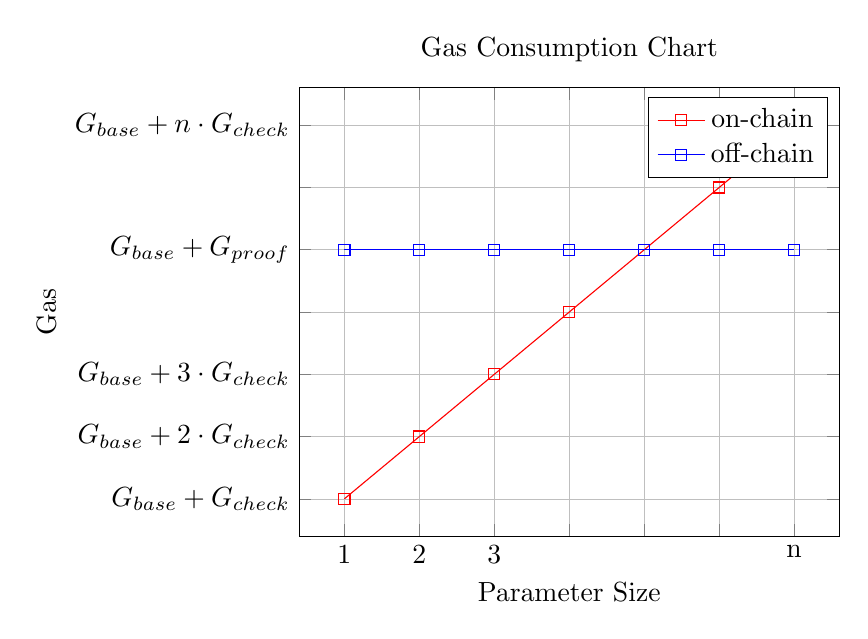
\begin{tikzpicture}
    \begin{axis}[
        title={Gas Consumption Chart},
        xlabel={Parameter Size},
        ylabel={Gas},
        grid=both,
        major grid style={line width=.2pt,draw=gray!50},
        minor grid style={line width=.1pt,draw=gray!20},
        xtick={1,2,3,4,5,6,7,8},
        xticklabels={1,2,3,,,,n,},
        ytick={1,2,3,4,5,6,7,8},
        yticklabels={$G_{base} + G_{check}$,$G_{base} + 2 \cdot G_{check}$, $G_{base} + 3 \cdot G_{check}$,,$G_{base}+ G_{proof}$,,$G_{base} + n \cdot G_{check}$,},
    ]
      \addplot[
        color=red,
        mark=square,
        ]
        coordinates {
        (1,1)(2,2)(3,3)(4,4)(5,5)(6,6)(7,7)
        };
        \addlegendentry{on-chain}
         \addplot[
        color=blue,
        mark=square,
        ]
        coordinates {
        (1,5)(2,5)(3,5)(4,5)(5,5)(6,5)(7,5)
        };
        \addlegendentry{off-chain}
    \end{axis}
  \end{tikzpicture}
  \caption{Gas Cost Comparison}
  \label{fig:gas_compare}
\end{figure}
\section{Prototype Implementations}
\label{sec:prototype-implementation}
This section presents the implementation of the Decentralized Selling Platform (DSP) application. Initially deployed as a smart contract on Ethereum for on-chain parameter verification, we demonstrate how off-chain verification reduces gas costs. The code is available at \cite{dsp}.

\subsection{Decentralized Selling Platform}
DSP provides a decentralized system for managing and trading items. Sellers create platforms, list items, and buyers can purchase them directly.

Each item includes: (1) \texttt{product}: The product name and producer, (2) \texttt{forSale}: Availability status, (3) \texttt{price}: The price in wei, and (4) \texttt{owner}: The current owner’s Ethereum address.

Key functions: \texttt{createSellingPlatform(items)} to create a platform with sorted items, and \texttt{buyItem(sellingPlatform, product)} to purchase items, transferring ownership and funds. Functions like \texttt{setForSale} and \texttt{setPrice} update sale status and price. Items can share the same product name but have different producers, and users can search by product name.

To optimize gas costs, the item list must be sorted by product name. If unsorted, all related operations will fail.
\subsection{Implementation with On-chain Parameter Verification}
Each seller manages their platform using a \texttt{mapping} linking their address to a list of items:
\begin{lstlisting}[numbers=none]
mapping(address => Item[]) public sellingPlatform;
\end{lstlisting}
The contract includes a function to check if items are sorted by name, using \texttt{compareStrings} to compare adjacent elements. If unsorted, it returns \texttt{false}; otherwise, \texttt{true}. The \texttt{createSellingPlatform} function calls this check before platform creation.
\subsection{Applying the Proposed Approach}
We define key components, such as the checkpoint formula for identifying unsorted items. The seed \( s \) is tied to the \( i \)-th item, the expected seeds \( m \) are estimated, and the target hash \( t \) is computed.

The on-chain assertion contract extends the DSP contract with functions like \texttt{rewardPrice} and \texttt{counterexamplePrice} for off-chain verification. When \texttt{createSellingPlatform} is invoked, the item list is submitted with a \texttt{timestamp} and \texttt{status} (initially \texttt{false}). The caller deposits funds, forfeited if the list is unsorted. If a counterexample is found, the record is deleted, and the caller is penalized. If verified, \texttt{status} changes to \texttt{true}, enabling further actions.

The contract includes \texttt{claimReward(sellingPlatform, seed)} to verify if a submission is a counterexample or valid proof.

The off-chain program, built in JavaScript with Ether.js, listens for platform submission events. It generates a random seed \( s \), used to find a counterexample or valid proof, then calls \texttt{claimReward} on-chain to claim the reward.
\subsection{Gas Savings}
We compared gas consumption between on-chain verification and the proposed off-chain approach based on item list size. Table \ref{gas-save} show that gas savings increase with list size; for example, an array of 50 items saves around 115,328 gas. Actual savings in tokens depend on the reward setup.

This smart contract can be optimized by using on-chain verification for small lists and off-chain for larger ones, achieving optimal gas efficiency.
\begin{table}[h]
\label{gas-save}
\centering
\caption{On-chain and Off-chain Parameter Verification Gas Comsuming}
\begin{tabular}{c|>{\centering\arraybackslash}p{3cm}|>{\centering\arraybackslash}p{3cm}|c}
\toprule
Parameter Size & On-chain & Off-chain & Gas save \\
\midrule
05  &  504225   &  578196   &  -73971   \\
10  &  903555   &  908838   &  -5283   \\
20  &  1842037  &  1804283  &  37754  \\
30  &  2797283  &  2733927  &  63356  \\
50  &  4708543  &  4593215  &  115328 \\
70  &  6714839  &  6545213  &  169626 \\
100 &  9581470  &  9333977  &  247493 \\
120 &  11492538 &  11193157 &  299381 \\
150 &  14359469 &  13981933 &  377536 \\
170 &  16270716 &  15841101 &  429615 \\
200 &  19137934 &  18629877 &  508057 \\
\bottomrule
\end{tabular}
\end{table}
\section{Related work}
\label{sec:related-work}
Smart contracts have been widely adopted to automate and secure decentralized applications. However, intensive on-chain computation can lead to high gas costs or exceed gas limits. To address this, many approaches focus on moving computations off-chain and distributing the verification process.

Layer 2 solutions like Plasma \cite{plasma-whitepaper} shift heavy computation to a child chain anchored to Ethereum Mainnet, improving scalability but not suited for parameter verification. More recently, optimistic rollups \cite{optimisticrollups} and zk-rollups \cite{zkrollups} emerged, offloading computation while preserving security. Optimistic rollups allow challenges via fraud proofs, similar to our counterexample mechanism, while zk-rollups use cryptographic proofs. However, both focus on transaction throughput, not complex parameter verification.

Decentralized oracle networks like Chainlink \cite{chainlink} enable off-chain data validation but are designed for fetching external data, not parameter verification. Their incentive model differs from our proof-of-work mechanism.

zk-SNARKs and zk-STARKs \cite{groth2016snarks} allow efficient on-chain verification but are computationally demanding, making them impractical for continuous validation. Privacy-focused solutions like Hawk \cite{7546538} leverage hybrid on-chain/off-chain computation, aligning with our approach. Arbitrum \cite{10.5555/3277203.3277305} also supports off-chain computation, but primarily at the consensus level.

Our work builds on these foundations by proposing a distributed, incentive-driven off-chain verification model to improve gas efficiency and enable counterexample searches. Unlike prior approaches, our method focuses on parameter verification using a distributed network of validators. The proof-of-work mechanism incentivizes validators, ensuring correctness without the high costs of on-chain verification.
\section{Conclusion}
\label{sec:conclusion}
This paper proposes a method for parameter verification in blockchain smart contracts by offloading expensive on-chain verification to an off-chain system, submitting only the results on-chain. We introduce an incentive mechanism to encourage validator participation while ensuring parameter correctness. Our gas cost analysis shows significant benefits, especially for large, costly parameters.

Future work includes developing an automated tool to convert heavy on-chain verification to the off-chain system, with a specification language for defining parameter properties, automatically generating smart contract functions and off-chain programs.
\newpage
\bibliographystyle{splncs04}
\bibliography{bio}
\end{document}
